\chapter{Method}\label{chp.method}

Three sections are included in this chapter. The experimental setup, the procedure of the experiment 
and the data processing procedures are introduced in details 
in Section~\ref{sec.method.setup},~\ref{sec.method.details} and~\ref{sec.method.postprocessing} respectively. 

\section{Experiment Setup}\label{sec.method.setup}
In this section, the enrollment of the participants, 
the stimuli and apparatus employed,
and the collection of the EMG data are introduced. 
The study described in this section is part of the parenthood study project supported by Deutsche Forschungsgesellschaft.
The experiment described in this section was conducted
in Psychology Institute of the Humboldt University in Campus Adlershof in Berlin. 

\textbf{Enrollment of the participants.}
In total, there were 62 female volunteers involved in our experiments by the time of writing, including 24 participants who were not raising a baby and constitute of the non-mother group, and 38 mothers who were breastfeeding a baby between two and six months and compose the mother group. Due to the problems of collected data, data from 17 non-mothers (aged 18-32, M = 24) was actually used. In order to compare the mothers and non-mothers, data from 20 mothers (aged 26-39, M = 31) was actually used.
All the participants received 40€ after the experiments for compensation.
To make sure the sanity of the collected data, telephone interviews 
were employed to screen the candidates using following criteria: A qualified participant should
\begin{itemize}
\item[-] be a female European descent for the sake of the facial expression recognition;
\item[-] be between 18 and 45 years old;
\item[-] be fluent in German, namely, on par with a native German speaker;
\item[-] not have taken medications which could influence the level of hormone;
\item[-] not have psychological disorder which could affect the perception or the production of facial expressions; 
\item[-] have normal or corrected-to-normal visual acuity.
\end{itemize}
Accordingly, all candidates were interviewed beforehand through a telephone call.
	
\textbf{The stimuli and the apparatus.}
Recall that,  
as introduced in Section~\ref{sec.hypothesis.expstrooptask},
the facial expressions from babies and from adults were employed as stimuli
in the extended Stroop task.
In particular, 
pictures include 
either positive (namely, smile) or negative (namely, cry or angry) facial expressions from 20 babies (ten girls and ten boys)\footnote{The pictures were collected from web and were rated to be highly related to the expressed emotions},
and from 20 adults (ten females and ten males)\footnote{The pictures come 
from Radboud Faces Database~\cite{langner2010presentation}.} were used.
All the pictures were normalized into a unified format to remove unrelated factors,
in terms of 
size (7cm $\times$ 9.33cm),
brightness, contrast grade (visual angle: 4.01\textdegree $\times$5.35\textdegree),
spatial frequency, and other properties. 
As for the text signals, 
German words Freude (happy) and Ärger (angry) were displayed in black color, 
superimposing on top of the facial pictures, indicating the same or the opposite facial expressions relative to the pictures. Four example pictures are displayed in Figure~\ref{fig.method.setup.example}, 
Both the facial pictures and the words were displayed in full screen on 19-inch monitors (35 cm $\times$ 25 cm), which was placed 70 cm away from the participants. 


\textbf{Record the responses from a participant.}
Different experiment conditions are summarized in Section~\ref{sec.hypothesis.design},
for which all trails were presented in random order, 
and at least 60 trials were collected for each experiment condition, 
ending up with 480 recorded trials in total.
The EMG signals from the participants
when making responses were captured. In addition,
videos of their facial expressions 
were also recorded to cross-examine the results derived from the EMG signals.
Based on the recorded EMG signals,
the response time was derived which will be introduced in Section~\ref{sec.method.postprocessing}. Besides, the electroencephalography (EEG) was also used to record the brain activity of the participants during the task, whose data was not analyzed in this work.

% and the accuracy of the response (e.g., a response is correct if it reflects the displayed word and verse visa.).

% In particular, the response from a participant
% is recored via electromyography (EMG)
% RT was measured as EMG onset latency of trials, 

%  During the experiment, the facial expressions of the participants were also recorded by the videos, which were used for double checking the quality of the data.
% RT was measured as EMG onset latency of trials, in which participants made the right facial expressions, and errors included no reactions, reactions using the incorrect muscle, or reactions were a response on both muscles in some of the trials according to the videos as well as EMG recording. The table 4.1 demonstrates the design of the experiment, showing all combinations of different factors.

\textbf{Locate and affix the electrodes for EMG recording.}
In the end, some details for recording the EMG signals are described. Recall that, as mentioned in Section~\ref{subsec.background.emg}, two electrodes were used for recording the signals from one target muscle, namely, two for the corrugator and two for the zygomaticus in our study, monitoring the muscle activity when particular facial expressions were made. Thereby, in total, four sintered silver-silver chlorid (Ag-AgCl) electrodes were in use.
Besides, 
a ground electrode is required in the EMG recording which was placed at the mid-line approximately 3-4 cm superior to the upper borders of the inner brows, akin to the configuration described in~\citep{fridlund1986guidelines}.

To attach the electrodes, 
the target skins were first 
cleaned with alcohol (Isopropylalcohol 70\%); thereafter the Electrolyte-Gel was peeled for 30 seconds to further reduce the resistance on the skin surface;
in the meantime, the head-shaped electrodes were filled with ``Abrasive Electrolyte-Gel'' without bubbles before attaching to skins using double-stick adhesive collars.  
To locate target muscles, 
we followed the descriptions from~\citep{fridlund1986guidelines}, namely,
for the corrugator, 
the participant was asked to frown and  
one electrode was affixed directly on the inner commossure of the eye fissure and another was positioned 1 cm lateral to, but slightly superior to, the first on the border of the eyebrow;
as for the zygomaticus, 
one electrode was attached on 
the midway along an imaginary line joining the corner of the mouth and the particular point on the right side, and another was placed 1 cm inferior and medial to the first (i.e. towards the mouth) along the same imaginary line (The positions of two electrodes and the ground electrode are illustrated in Figure~\ref{fig.background.emg}). The raw signal was digitized with the BrainVision recording software~\footnote{Brain Products GmbH, Munich, Germany}.
%The EMG signal was measured, rectified, and integrated using a Coulbourn V76-23a Hi amplifier. Low- and high-pass filters were set at $10 kHz$ and $8 Hz$, respectively. 
		

\begin{figure}[!t]
  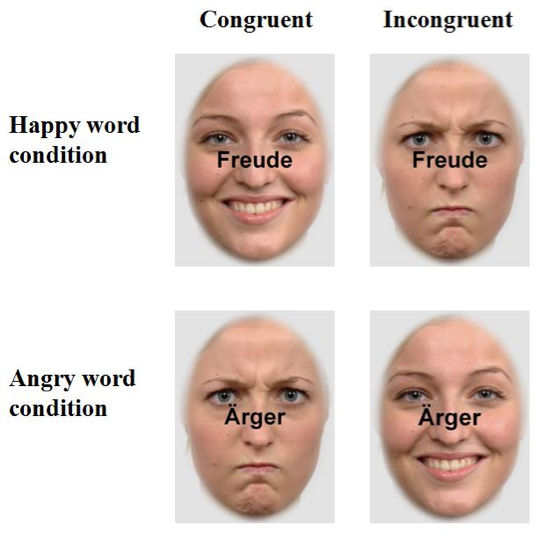
\includegraphics[width=0.9\linewidth]{pictures/Stimulus.png}
  \caption{An Example of face-word compound stimuli. The superimposing word indicates the requested facial expression from the participants, whereas the irrelevant facial pictures are displayed in the background. Up to the congruency between the word and the facial picture, there exist in total four combinations.
}
  \label{fig.method.setup.example}
\end{figure}


\section{Procedure}\label{sec.method.details}
In this section, 
the experiment details are 
described in sequence.


\noindent - \textbf{Before the task}, 
a participant was informed about the details via an information sheet, and was 
asked to complete a consent form and a demographic questionnaire (including a handedness questionnaire) whose templates are included in Appendix A and B respectively. Thereafter, the participant was seated on a comfortable chair in a soundproof and dimly-lit room. After the preparations of the electrodes, lasting about an hour, two other tasks were conducted for about a half hour before the Stroop task.

\noindent - \textbf{During the Stroop task,}
as explained in Section~\ref{sec.hypothesis.expstrooptask},
a participant was asked to response as soon as possible with a facial expression according to
the displayed word. They were also instructed to avoid making a hybrid
facial expression, namely, smiling and frowning at the same time,
which could result in invalid data.
Specifically, in each trial,
a fixation is first displayed for 500 ms,
thereafter, either ``Freude'' or ``Ärger'' is displayed in the center of 
a facial picture from a baby or from an adult with a positive or negative 
emotion for 2000 ms, during which the participant should response with 
a facial expression according to the word, until the sign ``stop'' is displayed when the participant should 
relax his(her) facial muscles returning to a neutral facial expression (an example is
displayed in Figure~\ref{fig.method.sequence});
% At the beginning of each trial, a fixation cross appeared on the screen for 500 ms. After the fixation, the face-word compound stimuli, namely a word ``happy'' or ``angry'' with either a `happy' or an `angry' facial expression of either baby or adult faces in the background, appeared in the center of the screen, which were visible for 2000 ms, during which participants could response to the words (i.e., Freude, Ärger) with facial expressions. When the `stop' signal appeared (900-1000 ms randomized), participants were instructed to relax their facial muscles and display neutral facial expression (see the Figure 4.3). 

\noindent - \textbf{Training and monitoring.}
Prior to the actual experiments, 
participants could familiarize themselves within the 
first eight trials, with which the EMG signals and the 
response patterns were also double-checked. 
During the tasks,
the procedure was monitored by our researchers from outside. Since the questionnaires for mothers are in terms of the baby, the mothers were asked to bring their baby with them to the lab. During the experiment, the babies were being taken cared and were outside the experimental room, avoiding 
their influences to the mothers from their own babies.
After every eighty trials, 
biscuits and water were offered to the participants for a break.


\noindent - \textbf{After the task,}
the second part of the questionnaire including two questions about the concentration and concerns during the Stroop task was filled (Appendix C for non-mothers and Appendix D for mothers). Each statement has four options: not at all, a little, quite and very. This self-evaluation of the concentration and concerns was used to cross examine the sanity of the data. The Stroop task (ca. 60‐min duration) was the third task, after which there was another task lasting for an hour. The whole experiment including the preparation and four tasks lasting for about four hours, including the pauses in between. At the end of the experiment, the participants were given 40€ as compensation.

% Abbildung 1

\begin{figure}[!t]
\centering
  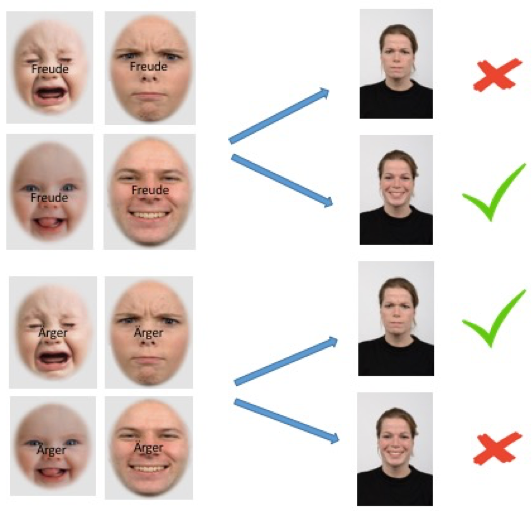
\includegraphics[width=0.9\linewidth]{pictures/Extended_Stroop_Task.png}
  \caption{Examples of the correct and wrong responses from a participant under different experiment conditions.
}
  \label{fig.method.task}
\end{figure}


\begin{figure}[!t]
  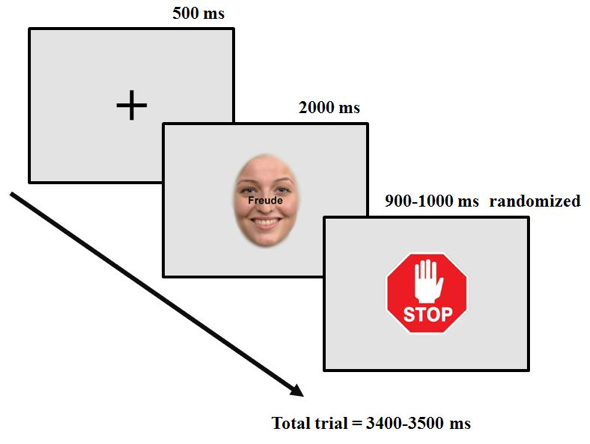
\includegraphics[width=0.9\linewidth]{pictures/One_Trial.png}
  \caption{Example of the sequences of scenes in one trial.
}
  \label{fig.method.sequence}
\end{figure}

\section{Data Processing}\label{sec.method.postprocessing}
\textbf{Post-processing of EMG data.}
Brain Vision Analyzer Software\footnote{Version 2.0, Brain Products Inc., Gilching, Germany} was used in the analyses of the EMG activity. 
The EMG signals were first filtered with a 50 Hz notch filter of the Zero Phase Shift Butterworth Filters (IIR Filters) to remove a narrow frequency band. 
The filtered EMG signals were further segmented. In particular, using the appearance of the 
stimulus, namely, the first occurrence of the word and the facial picture in a trial, as the~\textit{reference point}, and the interval between 200ms before and 2000ms after this reference was regarded as the span of the signal sequence in a trial. 
In measuring the activation of the muscles, 
in individual trials,
the strength of the signals on the first 200ms (namely, before the reference point) were regarded as baseline, corresponding to when no muscle activity presents.
According to the previous study~\citep{recio2014should}, a threshold relative to the baseline was determined by using the average strength plus 25 times of standard deviation,
which applied for all the participants. This threshold was used to determine the onset of activation of the target muscles, namely, the point in time where the amplitude in a given muscle reached 25\% of the individual maximal value of that muscle in the average was determined as the EMG onset for each trial~\citep{recio2014should}.


\textbf{Extraction of correctness.}
After processing the EMG, 
the triggered muscles, together with its activating time, were extracted, and associated
with the experiment conditions (namely, a particular type of stimulus).
Accordingly, 
the correctness of a recorded response 
could be determined by examining the EMG signals 
for the particular muscles and the displayed word, e.g., the response is correct if a EMG signal for the muscle zygomaticus exceeds the threshold while the one for the muscle corrugator doesn't, when the  ``Freude'' is displayed. 
Note that, 
if EMG signals for both muscles are below or above the threshold at the same time, the response is judged as incorrect.  

%was measured in some of the trials. There were two conditions when both muscles activated in the same time. In one condition, the wrong muscle activated first and then the right one. While in the other condition, the right muscle activated first and then the wrong one, indicating the uncertainty of the participants. The former was marked as wrong actions, while the latter was also marked as wrong actions for most of the participants in order to get the pure data. However, for nine participants (Seven mothers and two non-mothers) with more than 20 such trials, each trial was evaluated depending on the video recorded during the experiment.


\textbf{Extraction of response time.}
The latency of the first signal exceeding the 
threshold relative to the reference point was regarded as the response time.
According to the pilot experiments, 
a response time is valid only when it is between 70ms and 1000ms,
so that the erroneous records are filtered out. 
Intuitively, it is meaningful to analyze the 
response time only when a correct response presents, 
given that an incorrect response may due to a different mixture of conditions than a correct one.
Therefore, we did not want to mix up different kinds of processes and considered only the reaction time from correct trials.


\textbf{Statistic analysis.}
Given the extracted accuracy rate and the response time,  
statistical instruments were employed to examine the hypothesizes described in Section~\ref{sec.hypothesis}.
We first provide descriptives of the collected data by calculating 
several descriptive statistics. To start with, we confirmed that the collected accuracy and response time from different participants all centralize 
around the average, locating in the span between 
negative to positive
three standard deviation around the mean value. 
In addition, the average accuracies for individual participants over different experiment conditions (namely, for each participant, eight average accuracies were examined) are all above 0.5. Both observations indicate that
the participants understand the instructions well and adhere to them during the tasks.

In the following, the statistical tests are described, which are implemented with SPSS\footnote{IBM Corp. Released 2016. IBM SPSS Statistics for Windows, Version 24.0. Armonk, NY: IBM Corp.}. 
A significance level at 0.05 is reported in all tests.
% After each test, the descriptive statistics are analyzed, so that we could determine the direction of the differences.

%As a precondition of applying the mixed ANOVA, the between- and within-subjects are proved to be both independent and nominally scaled. The Greenhouse–Geisser adjustment is used to correct for violations of sphericity. There is homogeneity of the error variances, as assessed by Levene’s test (p > .05) and homogeneity of covariances, as assessed by Box’s test (p > .05). Alpha level of 0.05 is used to determine statistical significance. 
%As the premise of the experiment, we intend to examine that the Stroop effect exists in our study. Therefore, we first merge the $m1$, $m2$, $m7$, $m8$ as well as $n1$, $n2$, $n7$, $n8$ as the congruent conditions, and the $m3$, $m4$, $m5$, $m6$ as well as $n3$, $n4$, $n5$, $n6$ as incongruent conditions regardless of mothers and non-mothers. A paired t-test is conducted in order to investigate whether the Stroop effect is found.

\noindent - \textbf{Test for Stroop effect}.
Before examining the hypothesizes,
we first demonstrated the extended Stroop effect, namely,
among all trials,
a shorter (longer) response time and a higher (lower) accuracy rate
when the word and the facial expression are congruent(incongruent),
examining the designed extended Stroop task and the collected data.
A paired sample t-test was employed between 
$M_1\cup M_2\cup M_7\cup M_8\cup N_1\cup N_2\cup N_7\cup N_8$ and
$M_3\cup M_4\cup M_5\cup M_6\cup N_3\cup N_4\cup N_5\cup N_6$ from Table~\ref{sec.hypothesis.design},
where the congruency was considered as independent variable. 

\noindent - \textbf{Test for hypothesis 1}.
Recall that, in this hypothesis, we intend to investigate whether the Stroop effect is larger in the group of mother than of non-mother. Accordingly, an unpaired t-test was used, 
where the Stroop effect becomes the dependent variable and 
the status of motherhood (namely, being a mother or a non-mother) is an independent variable. 
Given the different sample sizes of the two groups (17 non-mothers and 20 mothers), 
the Welch's-test instead of the Student's t-test was employed. 
When further considering the types of the interferences, namely,
a positive (a smiling face) or a negative (a crying/frowning face), a Welch's test was also used to compare the difference of the Stroop effect between mother and non-mother when being provided a positive or a negative interference.

\noindent - \textbf{Test for hypothesis 2}.
Herein we intend to investigate whether the Stroop effect is larger when participants face the facial expressions from babies compared with when the adults' are displayed. A paired t-test was employed 
where the Stroop effect is the dependent variable, meanwhile the source of the interfering facial expression, namely a baby or an adult, is an independent variable. When combining the positive and negative interferences, we also investigated whether a negative or a positive interference from a baby leads to a larger Stroop effect compared to one from an adult using paired t-tests.


\noindent - \textbf{Test for hypothesis 3}.
In this hypothesis, a larger Stroop effect is expected 
when the mothers face the facial expressions from a baby. A paired t-test was used in the group of mother to compare the difference between the situations when the mothers are interfered by the babies and
by the adults, which was also conducted in the group of non-mother. We further consider the experiment conditions
when positive and negative interferences
were employed using paired t-test in the group of mother, namely, in front of a positive interference (smile), whether there is difference in the Stroop effect of a mother when the facial expression comes from a baby or an adult, meanwhile, whether the difference also exists, when being interfered by a negative one (frown or cry).

